\documentclass[a4paper,12pt]{extreport}

%====================== PACKAGES ======================
%%%%%%%%%%%%%%%%%%%%%%%%%%%%%%%%%%%%%%%%%
% Lachaise Assignment
% Structure Specification File
% Version 1.0 (26/6/2018)
%
% This template originates from:
% http://www.LaTeXTemplates.com
%
% Authors:
% Marion Lachaise & François Févotte
% Vel (vel@LaTeXTemplates.com)
%
% License:
% CC BY-NC-SA 3.0 (http://creativecommons.org/licenses/by-nc-sa/3.0/)
% 
%%%%%%%%%%%%%%%%%%%%%%%%%%%%%%%%%%%%%%%%%

%----------------------------------------------------------------------------------------
%	PACKAGES AND OTHER DOCUMENT CONFIGURATIONS
%----------------------------------------------------------------------------------------

\usepackage{amsmath,amsfonts,stmaryrd,amssymb} % Math packages

\usepackage{enumerate} % Custom item numbers for enumerations

\usepackage[ruled]{algorithm2e} % Algorithms

\usepackage[framemethod=tikz]{mdframed} % Allows defining custom boxed/framed environments

\usepackage{listings} % File listings, with syntax highlighting
\lstset{
	basicstyle=\ttfamily, % Typeset listings in monospace font
}

%----------------------------------------------------------------------------------------
%	DOCUMENT MARGINS
%----------------------------------------------------------------------------------------

\usepackage{geometry} % Required for adjusting page dimensions and margins

\geometry{
	paper=a4paper, % Paper size, change to letterpaper for US letter size
	top=2.5cm, % Top margin
	bottom=3cm, % Bottom margin
	left=2.5cm, % Left margin
	right=2.5cm, % Right margin
	headheight=14pt, % Header height
	footskip=1.5cm, % Space from the bottom margin to the baseline of the footer
	headsep=1.2cm, % Space from the top margin to the baseline of the header
	%showframe, % Uncomment to show how the type block is set on the page
}

%----------------------------------------------------------------------------------------
%	FONTS
%----------------------------------------------------------------------------------------

\usepackage[utf8]{inputenc} % Required for inputting international characters
\usepackage[T1]{fontenc} % Output font encoding for international characters

%\usepackage{XCharter} % Use the XCharter fonts

%----------------------------------------------------------------------------------------
%	COMMAND LINE ENVIRONMENT
%----------------------------------------------------------------------------------------

% Usage:
% \begin{commandline}
%	\begin{verbatim}
%		$ ls
%		
%		Applications	Desktop	...
%	\end{verbatim}
% \end{commandline}

\mdfdefinestyle{commandline}{
	leftmargin=10pt,
	rightmargin=10pt,
	innerleftmargin=15pt,
	middlelinecolor=black!50!white,
	middlelinewidth=2pt,
	frametitlerule=false,
	backgroundcolor=black!5!white,
	frametitle={Command Line},
	frametitlefont={\normalfont\sffamily\color{white}\hspace{-1em}},
	frametitlebackgroundcolor=black!50!white,
	nobreak,
}

% Define a custom environment for command-line snapshots
\newenvironment{commandline}{
	\medskip
	\begin{mdframed}[style=commandline]
}{
	\end{mdframed}
	\medskip
}

%----------------------------------------------------------------------------------------
%	FILE CONTENTS ENVIRONMENT
%----------------------------------------------------------------------------------------

% Usage:
% \begin{file}[optional filename, defaults to "File"]
%	File contents, for example, with a listings environment
% \end{file}

\mdfdefinestyle{file}{
	innertopmargin=1.6\baselineskip,
	innerbottommargin=0.8\baselineskip,
	topline=false, bottomline=false,
	leftline=false, rightline=false,
	leftmargin=2cm,
	rightmargin=2cm,
	singleextra={%
		\draw[fill=black!10!white](P)++(0,-1.2em)rectangle(P-|O);
		\node[anchor=north west]
		at(P-|O){\ttfamily\mdfilename};
		%
		\def\l{3em}
		\draw(O-|P)++(-\l,0)--++(\l,\l)--(P)--(P-|O)--(O)--cycle;
		\draw(O-|P)++(-\l,0)--++(0,\l)--++(\l,0);
	},
	nobreak,
}

% Define a custom environment for file contents
\newenvironment{file}[1][File]{ % Set the default filename to "File"
	\medskip
	\newcommand{\mdfilename}{#1}
	\begin{mdframed}[style=file]
}{
	\end{mdframed}
	\medskip
}

%----------------------------------------------------------------------------------------
%	NUMBERED QUESTIONS ENVIRONMENT
%----------------------------------------------------------------------------------------

% Usage:
% \begin{question}[optional title]
%	Question contents
% \end{question}

\mdfdefinestyle{question}{
	innertopmargin=1.2\baselineskip,
	innerbottommargin=0.8\baselineskip,
	roundcorner=5pt,
	nobreak,
	singleextra={%
		\draw(P-|O)node[xshift=1em,anchor=west,fill=white,draw,rounded corners=5pt]{%
		Question \theQuestion\questionTitle};
	},
}

\newcounter{Question} % Stores the current question number that gets iterated with each new question

% Define a custom environment for numbered questions
\newenvironment{question}[1][\unskip]{
	\bigskip
	\stepcounter{Question}
	\newcommand{\questionTitle}{~#1}
	\begin{mdframed}[style=question]
}{
	\end{mdframed}
	\medskip
}

%----------------------------------------------------------------------------------------
%	WARNING TEXT ENVIRONMENT
%----------------------------------------------------------------------------------------

% Usage:
% \begin{warn}[optional title, defaults to "Warning:"]
%	Contents
% \end{warn}

\mdfdefinestyle{warning}{
	topline=false, bottomline=false,
	leftline=false, rightline=false,
	nobreak,
	singleextra={%
		\draw(P-|O)++(-0.5em,0)node(tmp1){};
		\draw(P-|O)++(0.5em,0)node(tmp2){};
		\fill[black,rotate around={45:(P-|O)}](tmp1)rectangle(tmp2);
		\node at(P-|O){\color{white}\scriptsize\bf !};
		\draw[very thick](P-|O)++(0,-1em)--(O);%--(O-|P);
	}
}

% Define a custom environment for warning text
\newenvironment{warn}[1][Warning:]{ % Set the default warning to "Warning:"
	\medskip
	\begin{mdframed}[style=warning]
		\noindent{\textbf{#1}}
}{
	\end{mdframed}
}

%----------------------------------------------------------------------------------------
%	INFORMATION ENVIRONMENT
%----------------------------------------------------------------------------------------

% Usage:
% \begin{info}[optional title, defaults to "Info:"]
% 	contents
% 	\end{info}

\mdfdefinestyle{info}{%
	topline=false, bottomline=false,
	leftline=false, rightline=false,
	nobreak,
	singleextra={%
		\fill[black](P-|O)circle[radius=0.4em];
		\node at(P-|O){\color{white}\scriptsize\bf i};
		\draw[very thick](P-|O)++(0,-0.8em)--(O);%--(O-|P);
	}
}

% Define a custom environment for information
\newenvironment{info}[1][Info:]{ % Set the default title to "Info:"
	\medskip
	\begin{mdframed}[style=info]
		\noindent{\textbf{#1}}
}{
	\end{mdframed}
}
 % Include the file specifying the document structure and custom commands
\usepackage{graphicx}
\usepackage{gensymb}
\usepackage{float}
\usepackage[french]{babel}
\usepackage{comment}

%\usepackage[utf8x]{inputenc}
%pour les informations sur un document compilé en PDF et les liens externes / internes
\usepackage{hyperref}
%pour la mise en page des tableaux
%\usepackage{array}
%\usepackage{tabularx}
%pour utiliser \floatbarrier
%\usepackage{placeins}
%\usepackage{floatrow}
%espacement entre les lignes
%\usepackage{setspace}
%modifier la mise en page de l'abstract
\usepackage{abstract}
%police et mise en page (marges) du document
%\usepackage[T1]{fontenc}
%\usepackage[top=2cm, bottom=2cm, left=2cm, right=2cm]{geometry}



%====================== INFORMATION ET REGLES ======================

%rajouter les numérotation pour les \paragraphe et \subparagraphe
\setcounter{secnumdepth}{4}
\setcounter{tocdepth}{4}

\hypersetup{							% Information sur le document
pdfauthor = {Premier Auteur,
			Deuxième Auteur,
			Troisième Auteur,
    		Quatrième Auteur},			% Auteurs
pdftitle = {Nom du Projet -
			Sujet du Projet},			% Titre du document
pdfsubject = {Intern Report},		% Sujet
pdfkeywords = {Tag1, Tag2, Tag3, ...},	% Mots-clefs
pdfstartview={FitH}}					% ajuste la page à la largueur de l'écran
%pdfcreator = {MikTeX},% Logiciel qui a crée le document
%pdfproducer = {}} % Société avec produit le logiciel

%======================== DEBUT DU DOCUMENT ========================

\begin{document}

%régler l'espacement entre les lignes
\newcommand{\HRule}{\rule{\linewidth}{0.5mm}}

%page de garde
\begin{titlepage}
\begin{center}

% Upper part of the page. The '~' is needed because only works if a paragraph has started.

\includegraphics[width=0.15\textwidth]{./images/logo-ensea.png}~\\[1cm]

\textsc{\Large  Ecole nationale supérieure de l'électronique et de ses applications}\\[0.5cm]

% Title
\HRule \\[0.4cm]

{\huge \bfseries RAPPORT PLT\\
Réalisation d'un T-RPG type Disgaea   \\[0.4cm] }

\HRule \\[1.5cm]

% Author and supervisor
\begin{minipage}{0.4\textwidth}
\begin{flushleft} \large
\emph{Authors:}\\
Benjamin \textsc{Anslot}\\
Mathieu \textsc{Hadjadji}
\end{flushleft}
\end{minipage}
\begin{minipage}{0.4\textwidth}
\begin{flushright} \large


\emph{Années:} \\
2019 - 2020 \\
OPTION IS \\
\end{flushright}
\end{minipage}

\vfill

% Bottom of the page
{\large \today}

\end{center}
\end{titlepage}

%page blanche
\newpage
~
%ne pas numéroter cette page
\thispagestyle{empty}
\newpage

% \renewcommand{\abstractnamefont}{\normalfont\Large\bfseries}
%\renewcommand{\abstracttextfont}{\normalfont\Huge}

\begin{abstract}
\hskip7mm

%\begin{spacing}{1.3}

[Le résumé du projet]

%\end{spacing}
\end{abstract}

%\newpage


\tableofcontents
\thispagestyle{empty}
\setcounter{page}{0}
%ne pas numéroter le sommaire

% \newpage

%espacement entre les lignes d'un tableau
\renewcommand{\arraystretch}{1.5}

%====================== INCLUSION DES PARTIES ======================

~
\thispagestyle{empty}
%recommencer la numérotation des pages à "1"
\setcounter{page}{0}
\newpage

% \input{./acknowledgments.tex}
\chapter{Présentation Générale}



\section{Archétype}

L'objectif est de réaliser un jeu video de type Tactical RPG dans l'idée du jeu Disgaea.


\begin{figure}[H]
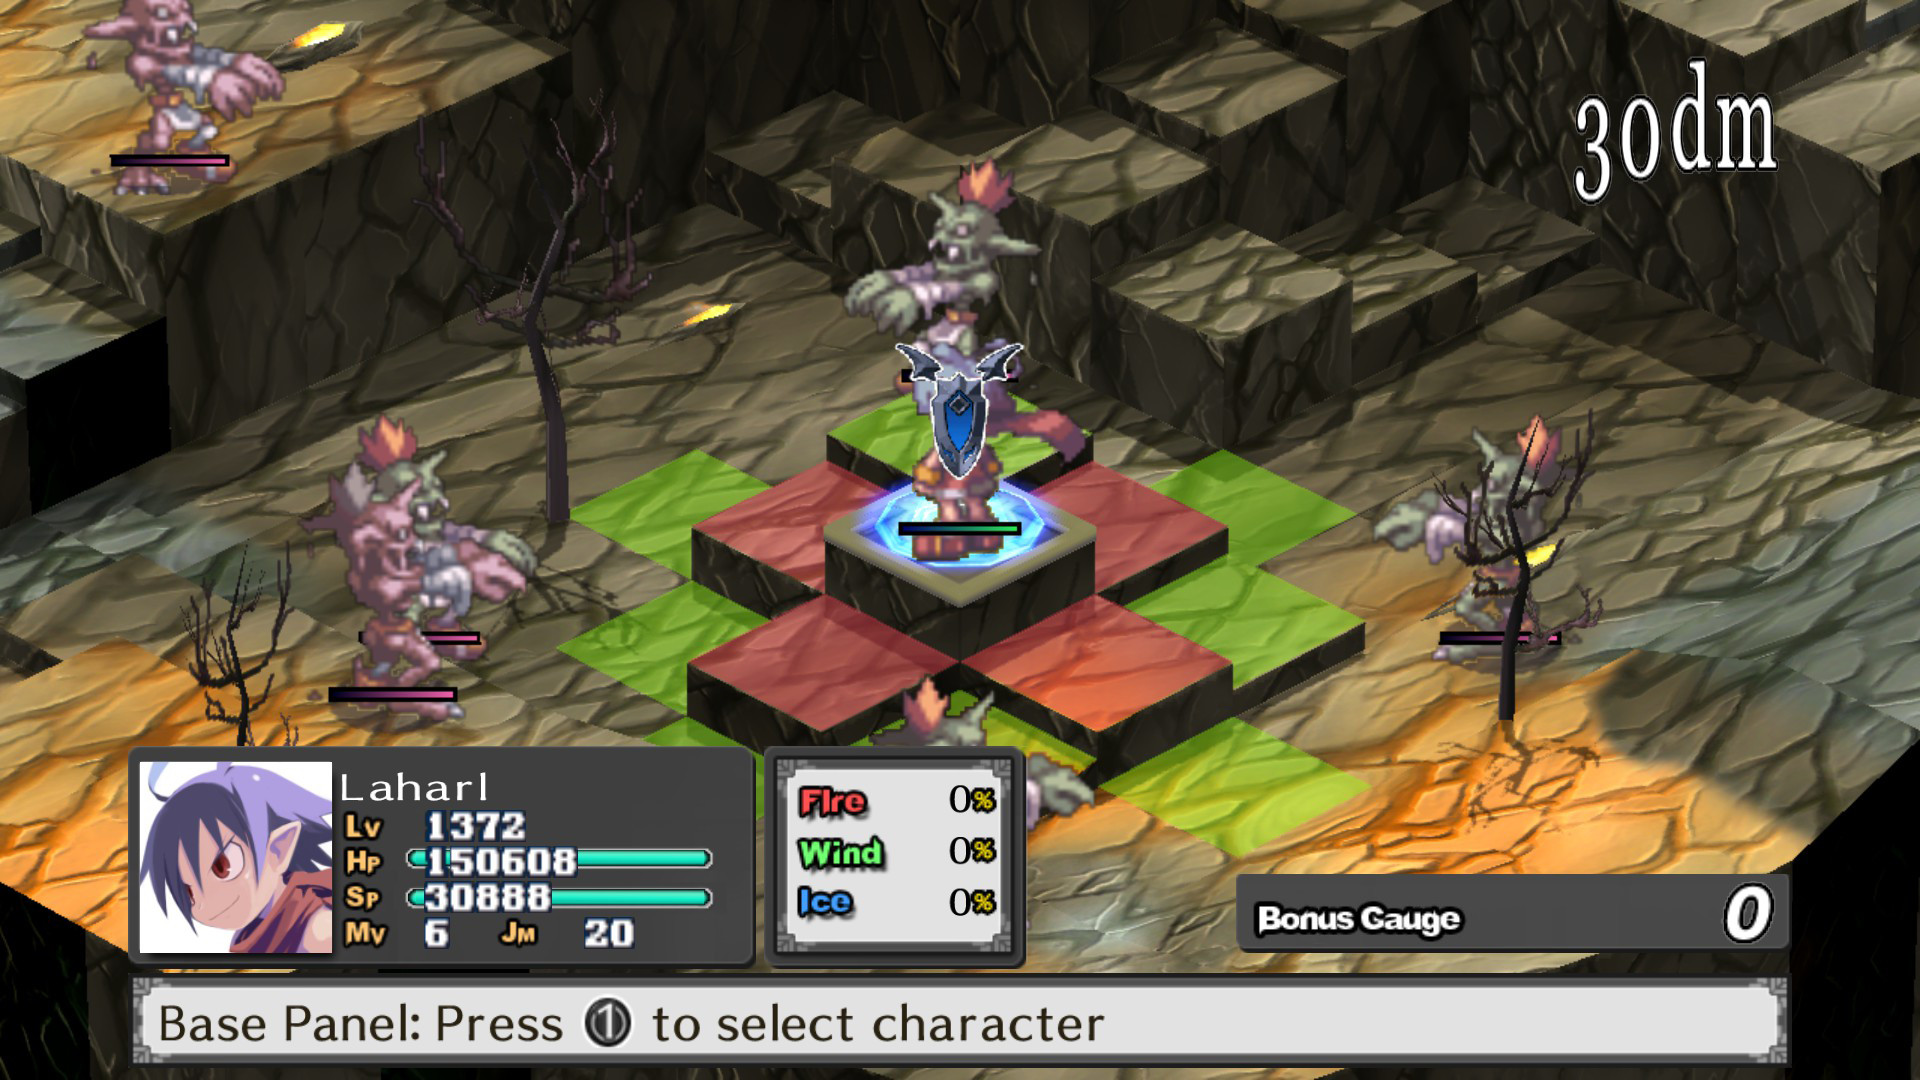
\includegraphics[width=\linewidth]{images/disgaea_exemple.png}
\centering
\caption{Aperçu de l'ecran de Jeu du jeu Disgaea}
\label{fig:img1}
\end{figure}



\section{Règles du Jeu}


\subsection{But du Jeu}
Les joueurs ont chacun un nombre défini de troupes positionné sur la carte.
Le But du jeu est d'éliminer l'ensemble des troupes ennemies (condition de victoire).
Ou d'avoir toutes ses troupes éliminées (condition de défaite).
\\
Une unité est considérée comme détruire lorsque ses points de vie tombent à 0.

\subsection{Tour de Jeu}
Le jeu se découpe en une sucession de tours. Les joueurs jouent les uns à la suite des autres.

Dans un tour, le joueur peut: \\

\begin{itemize}
  \item Déplacer ses unités sur la carte sur un nombre limité de cases.
  \item Attaquer avec ses unités des unités adverses adjacentes ou à distance en fonction du type d'attaque utilisable par l'unité. 
  \item Appliquer une posture de défense sur ses unités pour augmenter la défense si attaquée. 
  \item Utiliser des objets sur ses unités pour la soigner etc...

\end{itemize}

\subsection{Terrain de Jeu}

Le terrain est décomposé en tuiles. Une unité reçoit des bonus ou des malus en fonction de la tuile sur laquelle elle se trouve. Une unité placée sur une tuile de forêt par exemple recevra un bonus d'esquive si attaquée.\\

Les tuiles peuvent avoir des hauteurs différentes. Une unité placée sur une tuile en hauteur aura une meilleure portée pour des attaques à distance, mais y accèder coûte plus de points de déplacement.

\section{Ressources}

\begin{figure}[H]
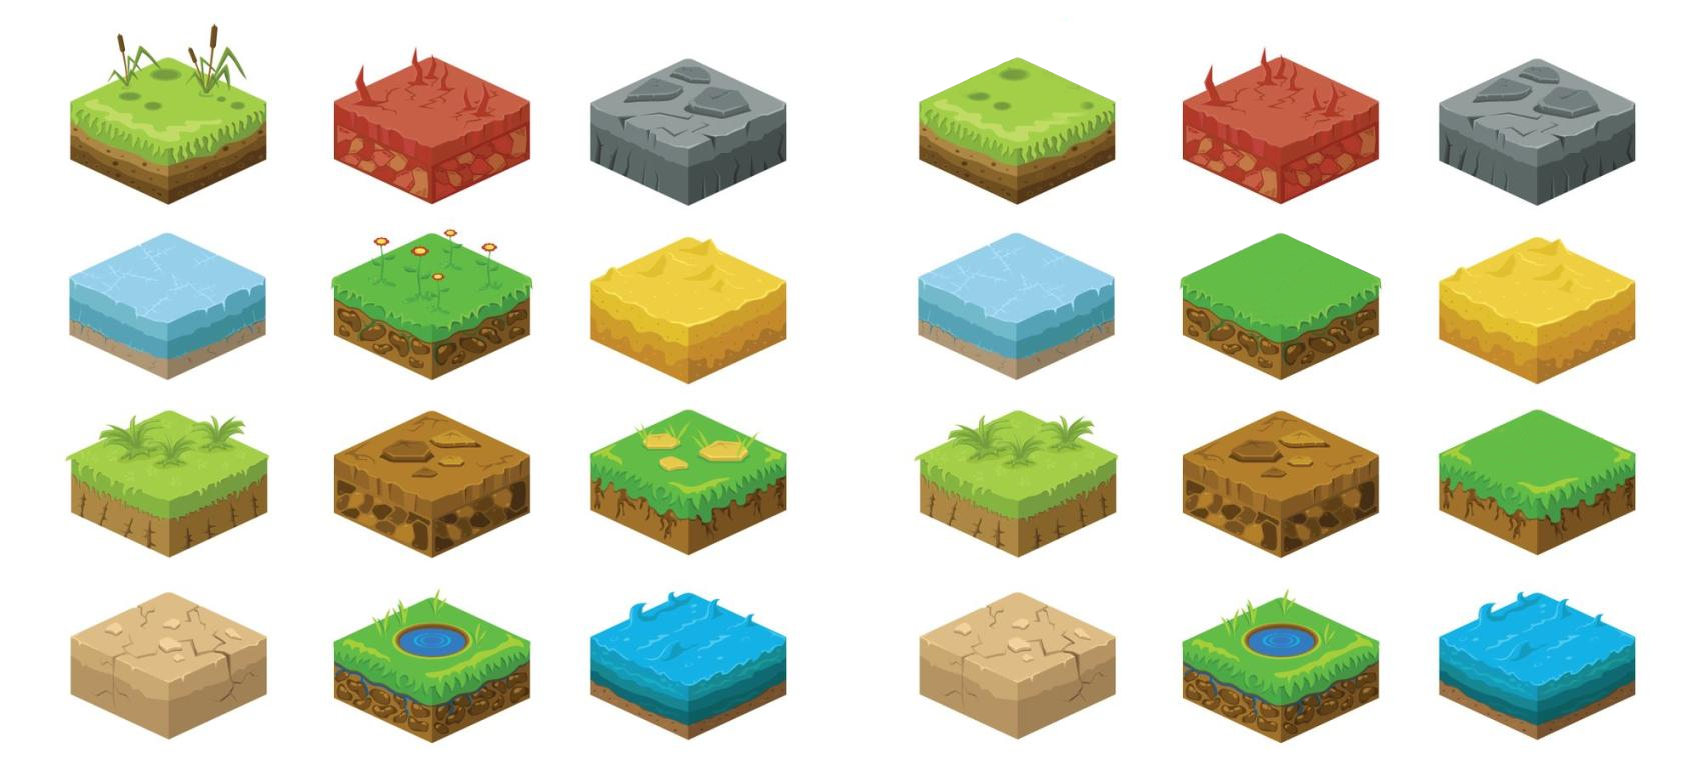
\includegraphics[width=\linewidth]{images/maptiles.png}
\centering
\caption{Tiles pour la carte en perspective isométrique}
\label{fig:img2}
\end{figure}

\begin{figure}[H]
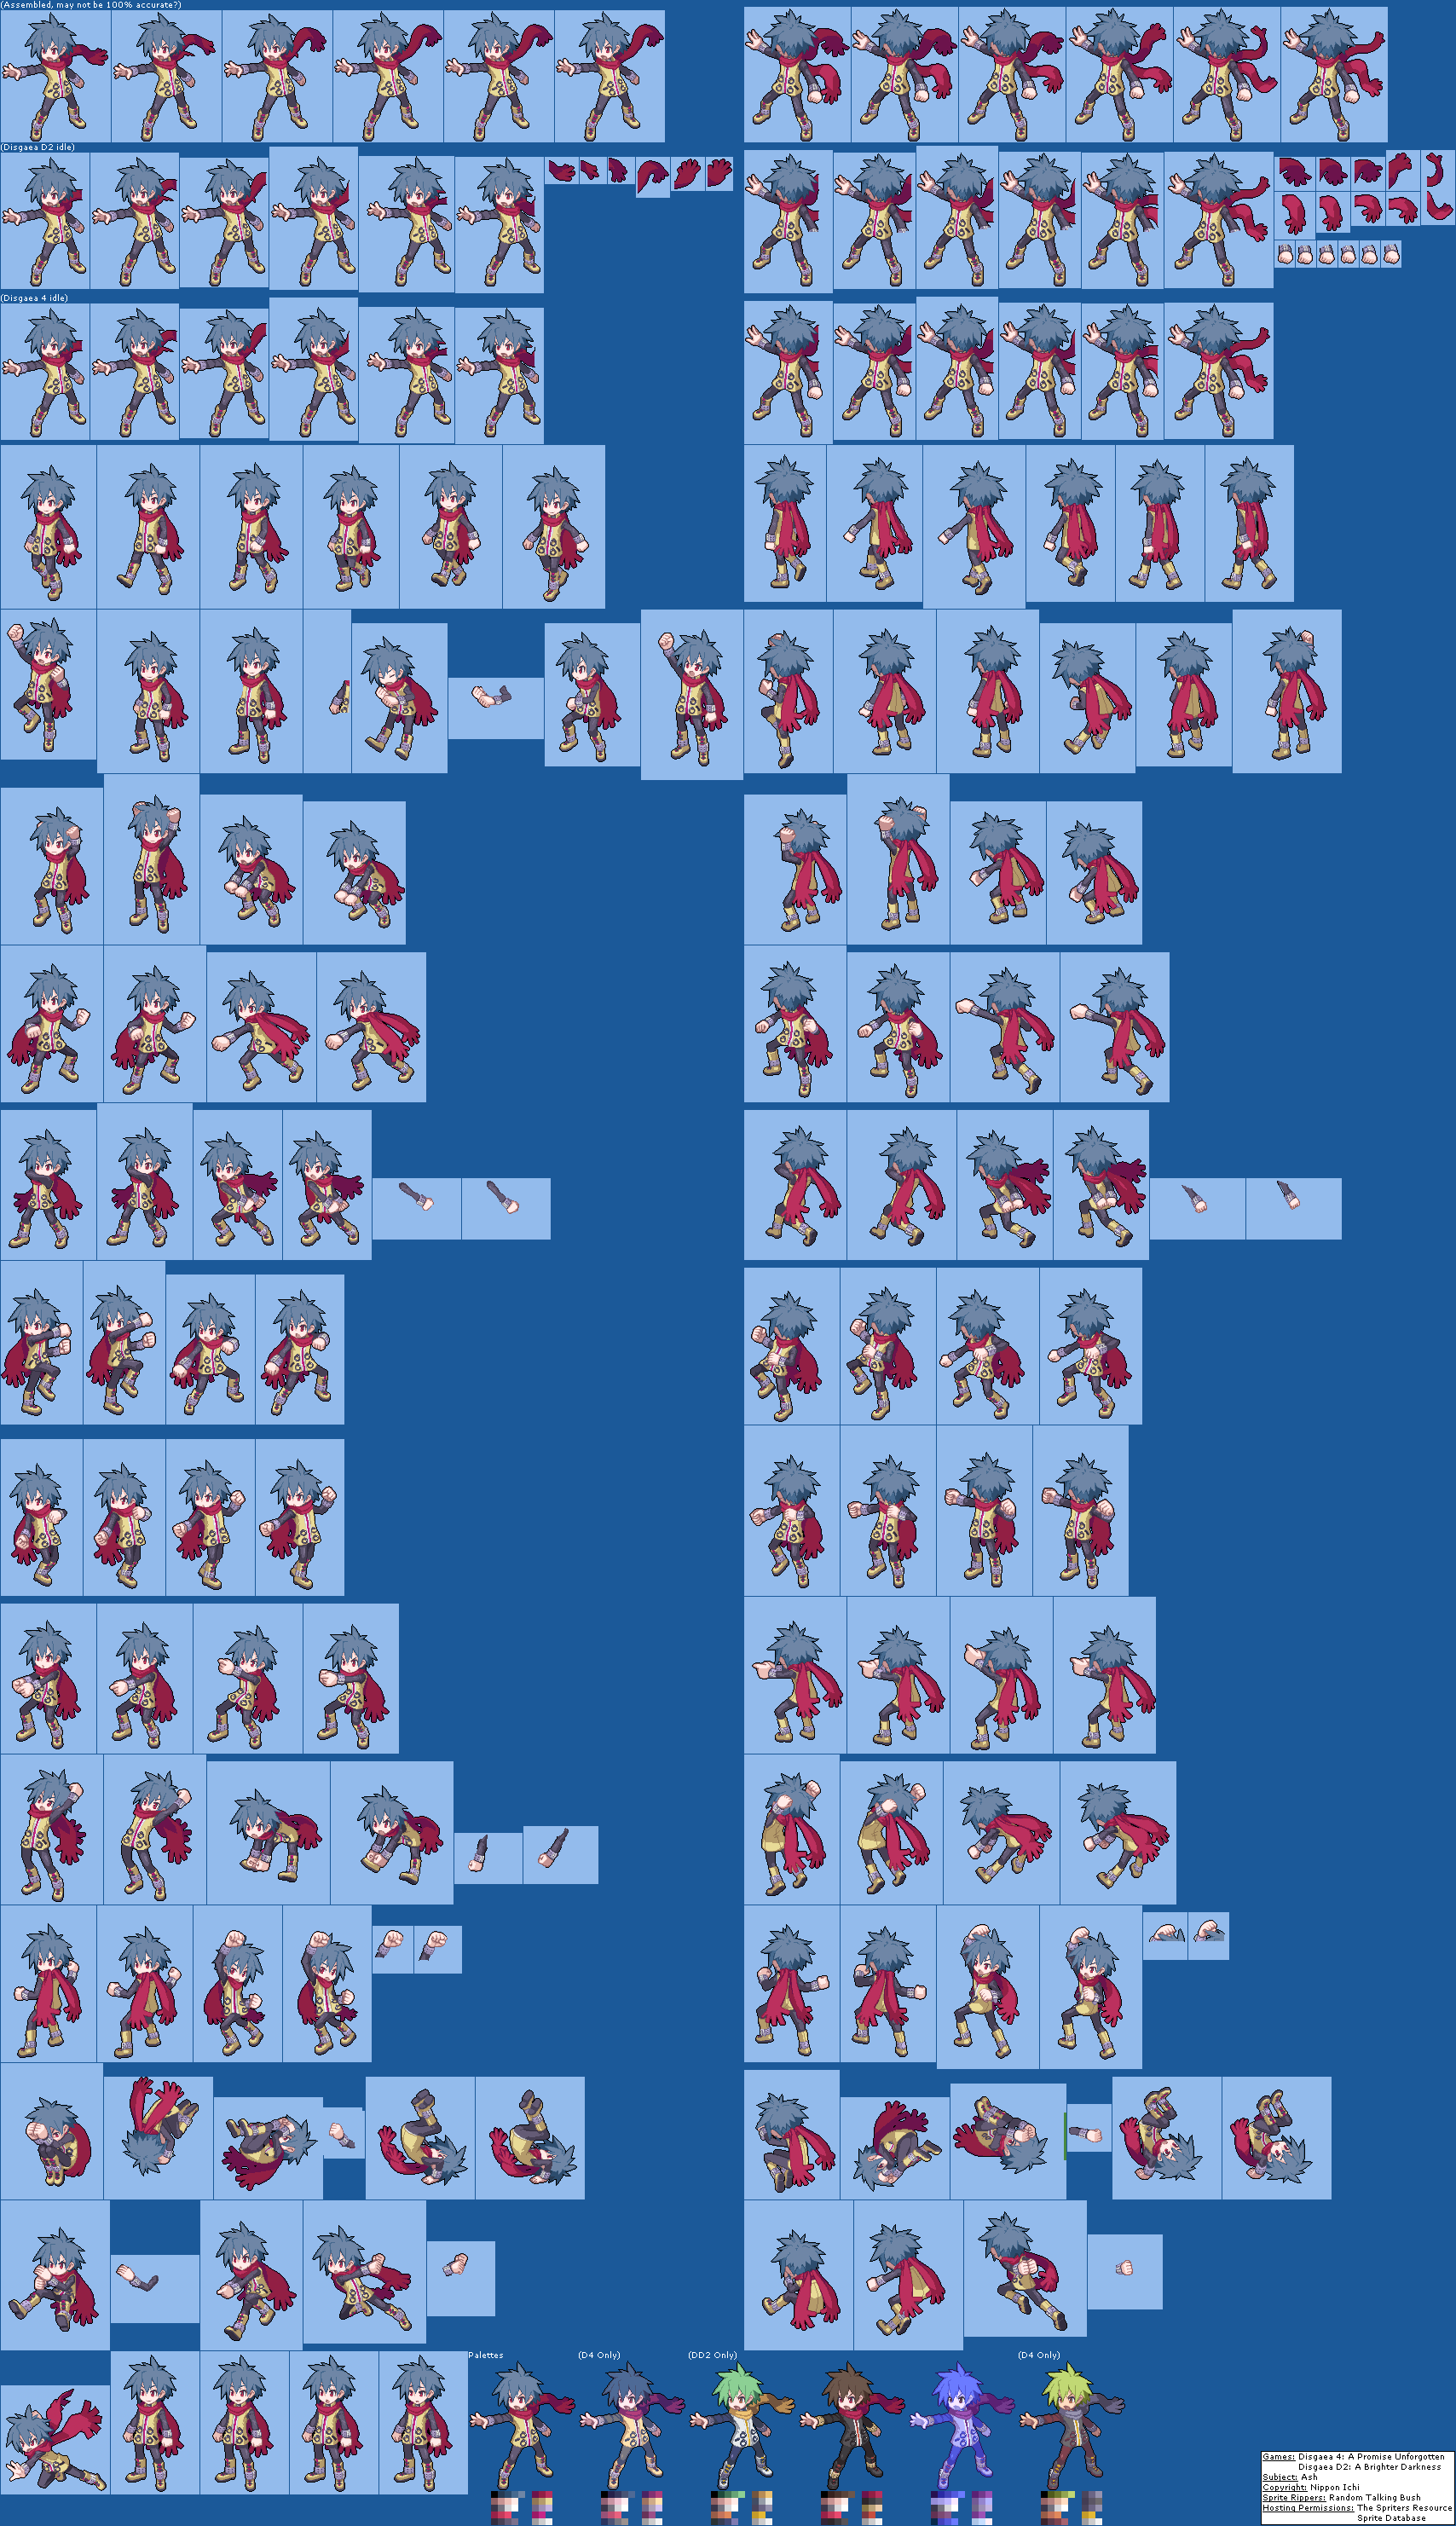
\includegraphics[scale=0.15]{images/char1.png}
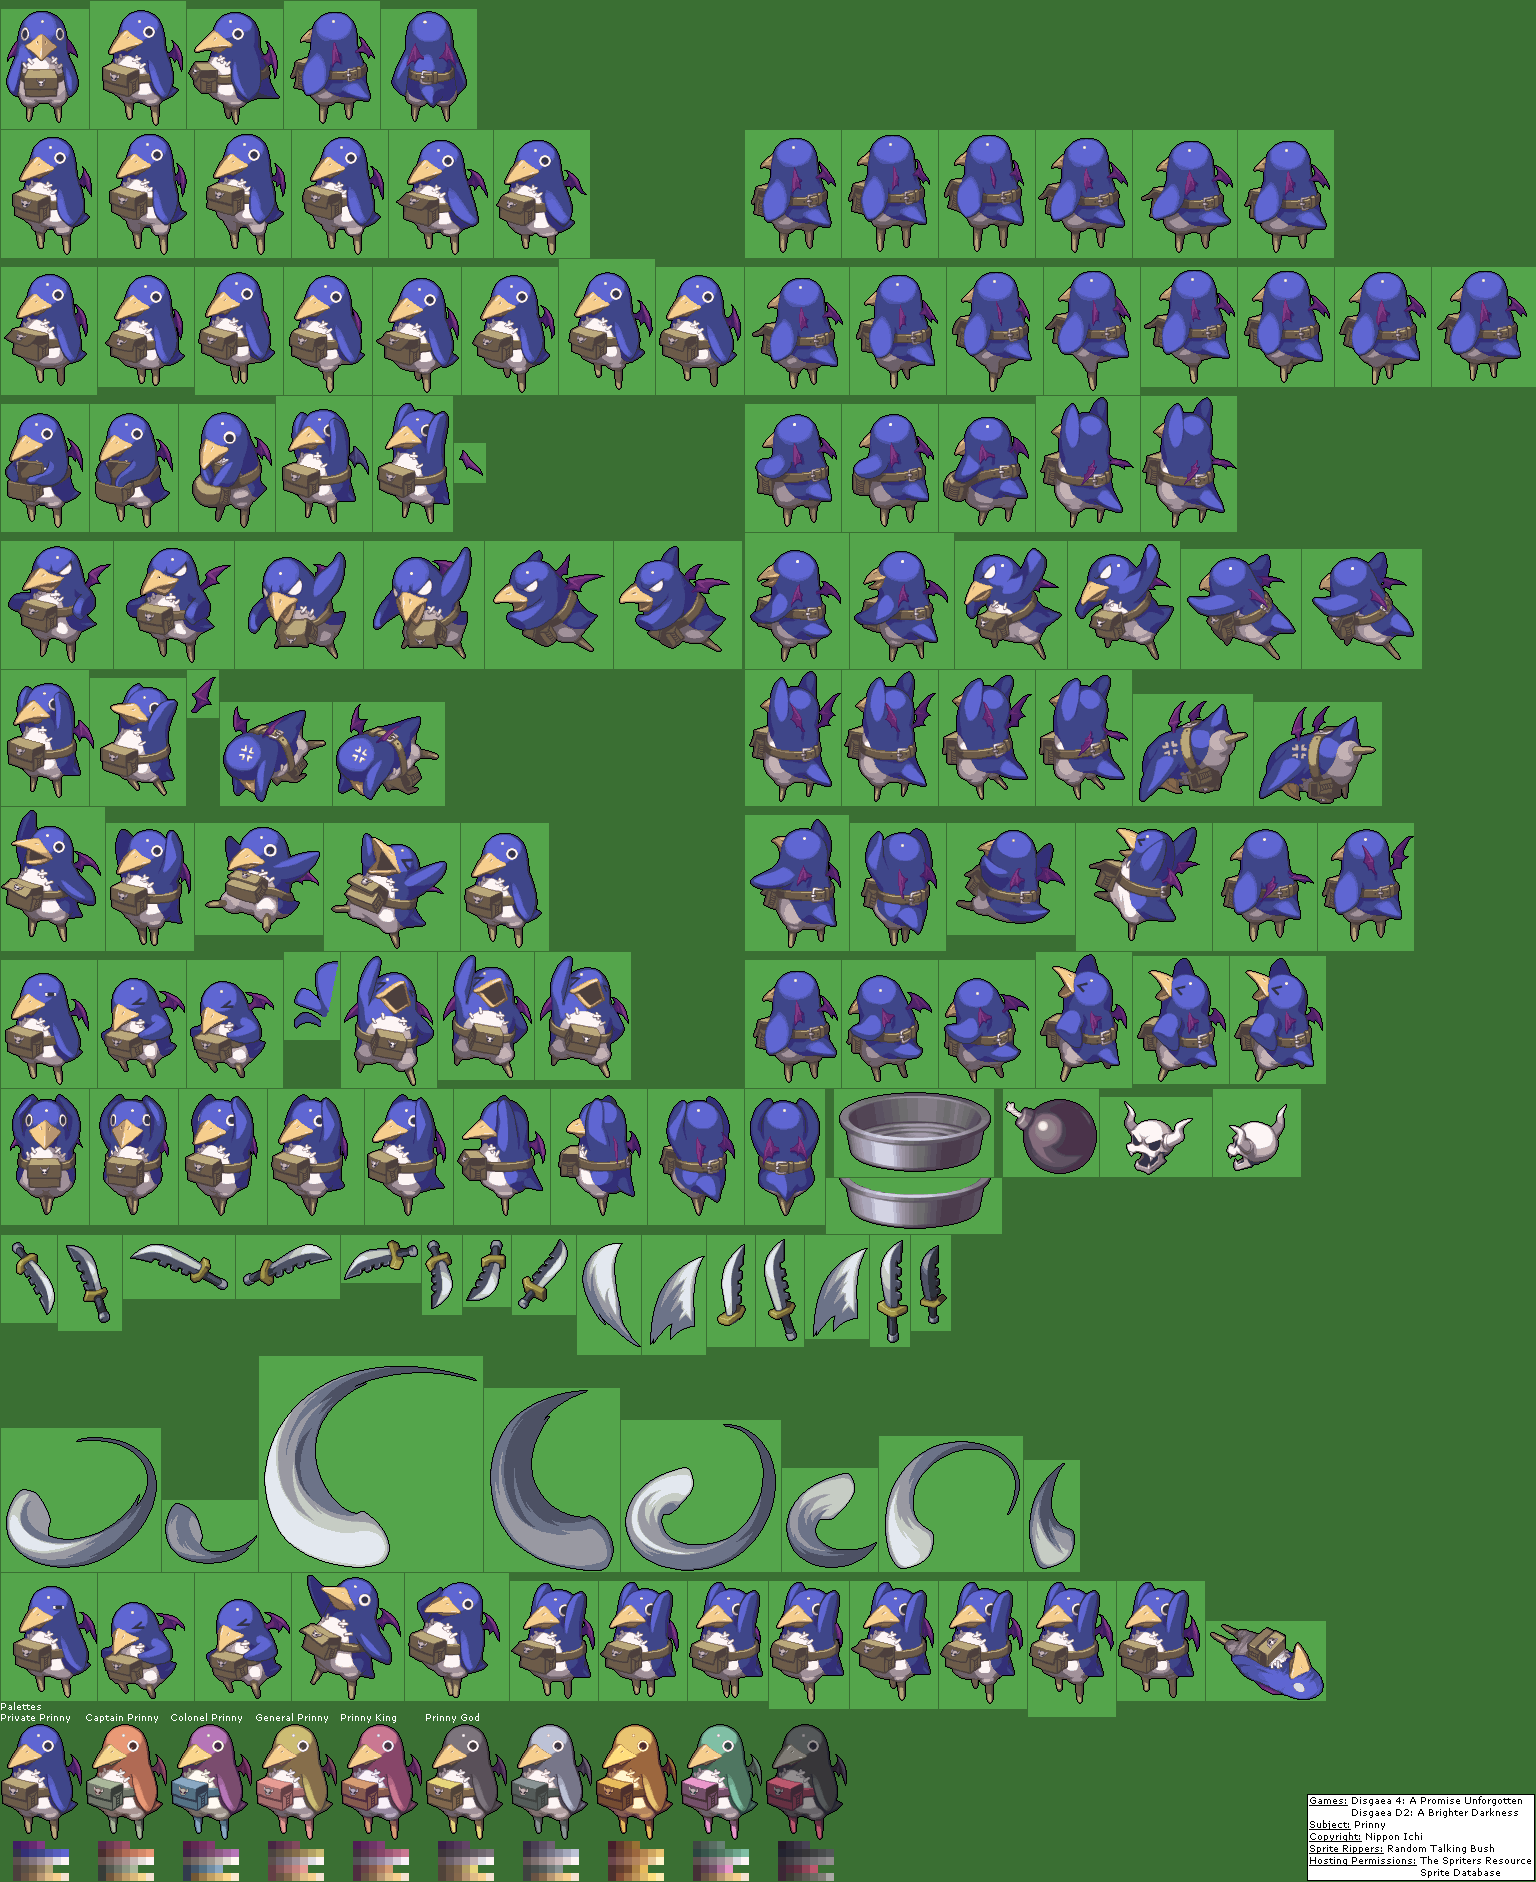
\includegraphics[scale=0.15]{images/enn1.png}
\centering
\caption{Spritesheets personnages}
\label{fig:img3}
\end{figure}

\chapter{Description et Conception des états}


\section{Description des états}

Dans un état du jeu, on retrouve des éléments fixes: les tiles (tuiles isometriques) qui composent la carte et des éléments mobiles: les personnages. Tous les éléments ont un nom et une position.

\subsection{Etat éléments fixes}

La carte du jeu est une table à 2 dimensions composée de tuiles.

Les tuiles sont générées de manière aléatoires. 
On retrouve dans les propriétés des tuiles : 
\\

\begin{itemize}
    \item \textbf{le type de tuile:} Il est critère de praticabilité pour un personnage et aussi pour l'affichage du sprite correspondant côté gestion rendu.
       \begin{itemize}
         \item[•]  Dirt
         \item[•]  Grass
         \item[•]  Water
         \item[•]  Sand
         \item[•]  Pound
         \item[•]  Rock
         \\
       \end{itemize}
    Les effets des types seront déterminés côté engine en fonction du type de tuile.
    \\
    \item \textbf{la hauteur:} Elle determine la hauteur de la tuile, modifieur impactant la distance de déplacement dans les actions et la portée d'une attaque qui seront gérés dans la partie engine. La hauteur est un entier compris entre 1 et 3.
\end{itemize}

\subsection{Etat éléments mobiles}

Les personnages appatiennent à des équipes. Chaque équipe est gérée par un joueur.  
Un personnage possède:
\\
\begin{itemize}
\item Une race générée aléatoirement parmi la liste suivante:
    \begin{itemize}
         \item[•]  Monster
         \item[•]  Beastman
         \item[•]  Demon
         \item[•]  Human
         \\
     \end{itemize}

\item Un job généré aléatoirement parmi la liste suivante:
    \begin{itemize}
         \item[•]  Pugilist
         \item[•]  Swordsman
         \item[•]  Archer
         \item[•]  Magician
         \\
     \end{itemize}
\item Un niveau calculé en fonction de l'expérience amassée.
\\ \\
Les caractéristiques (PV max, PM max, dégâts physiques, dégâts magiques, score d'évasion, score de défense, liste des compétences) sont déterminés en fonctions des 3 attributs précédents (race,job et niveau).
\\
\end{itemize}

Un curseur permet aux joueurs de navigueur sur les tuiles et lire les propriétés 
(du terrain et d'un personnage si présent) et sélectionner un personnage (si présent) en vue d'effectuer une action.


\subsection{Etat général}
En plus des éléments statiques et mobiles nous avons :
\begin{itemize}
         \item \textbf{nombre de tour:} Le nombre de tours qui ont été joués.
         \\
         \item \textbf{terminé:} Un booléen qui indique si le combat est terminé.
\end{itemize}

\section{Conception Logiciel}
Le diagramme des classes UML C++ pour les états est visible en Figure X. Nous pouvons mettre en évidence plusieurs groupes de classes qui sont les suivants :
\\
\begin{itemize}
    \item Groupe Character (bleu foncé): Toutes les charactéristiques des personnages, qu'ils soient ceux du joueur ou non, ainsi que les fonctions pour y accéder. Il présente une hiérarchie des classes filles permettant de visualiser les différentes catégories associées aux personnages et les types de chacun de ses élements.
    \\
    \item Groupe Team (bleu clair): Principalement composé de la classe Team, cette dernière englobe les ressources d'un joueur à savoir ses personnages et ses objets.
    \\
    \item Groupe Entity (jaune): La gestion du curseur et de l'entité pointée par ce dernier pour afficher les propriétés de la tuile à l'écran et selectionner le personnage qui réalise une action. 
    \\
    \item Groupe Observante (orange): Il sera implémenté en parallèle avec le render, pour pouvoir faire les tests.
    \\
    \item Groupe Turn (vert): Il représente l'état général durant un tour.
    \\
    \item Groupe Tile (gris): Ce groupe permet la construction d'une Tile aléatoire à l'aide de TileFactory. La carte sera formée à partir de ces Tiles. 
\end{itemize}

\section{Tests Unitaires}

Des tests unitaires ont été réalisés pour vérifier les fonctions des différentes classes. On réalise un fichier de test par classe.
Le code est couvert aux alentours de 88\% par les tests unitaires.

\newpage

\begin{figure}[H]
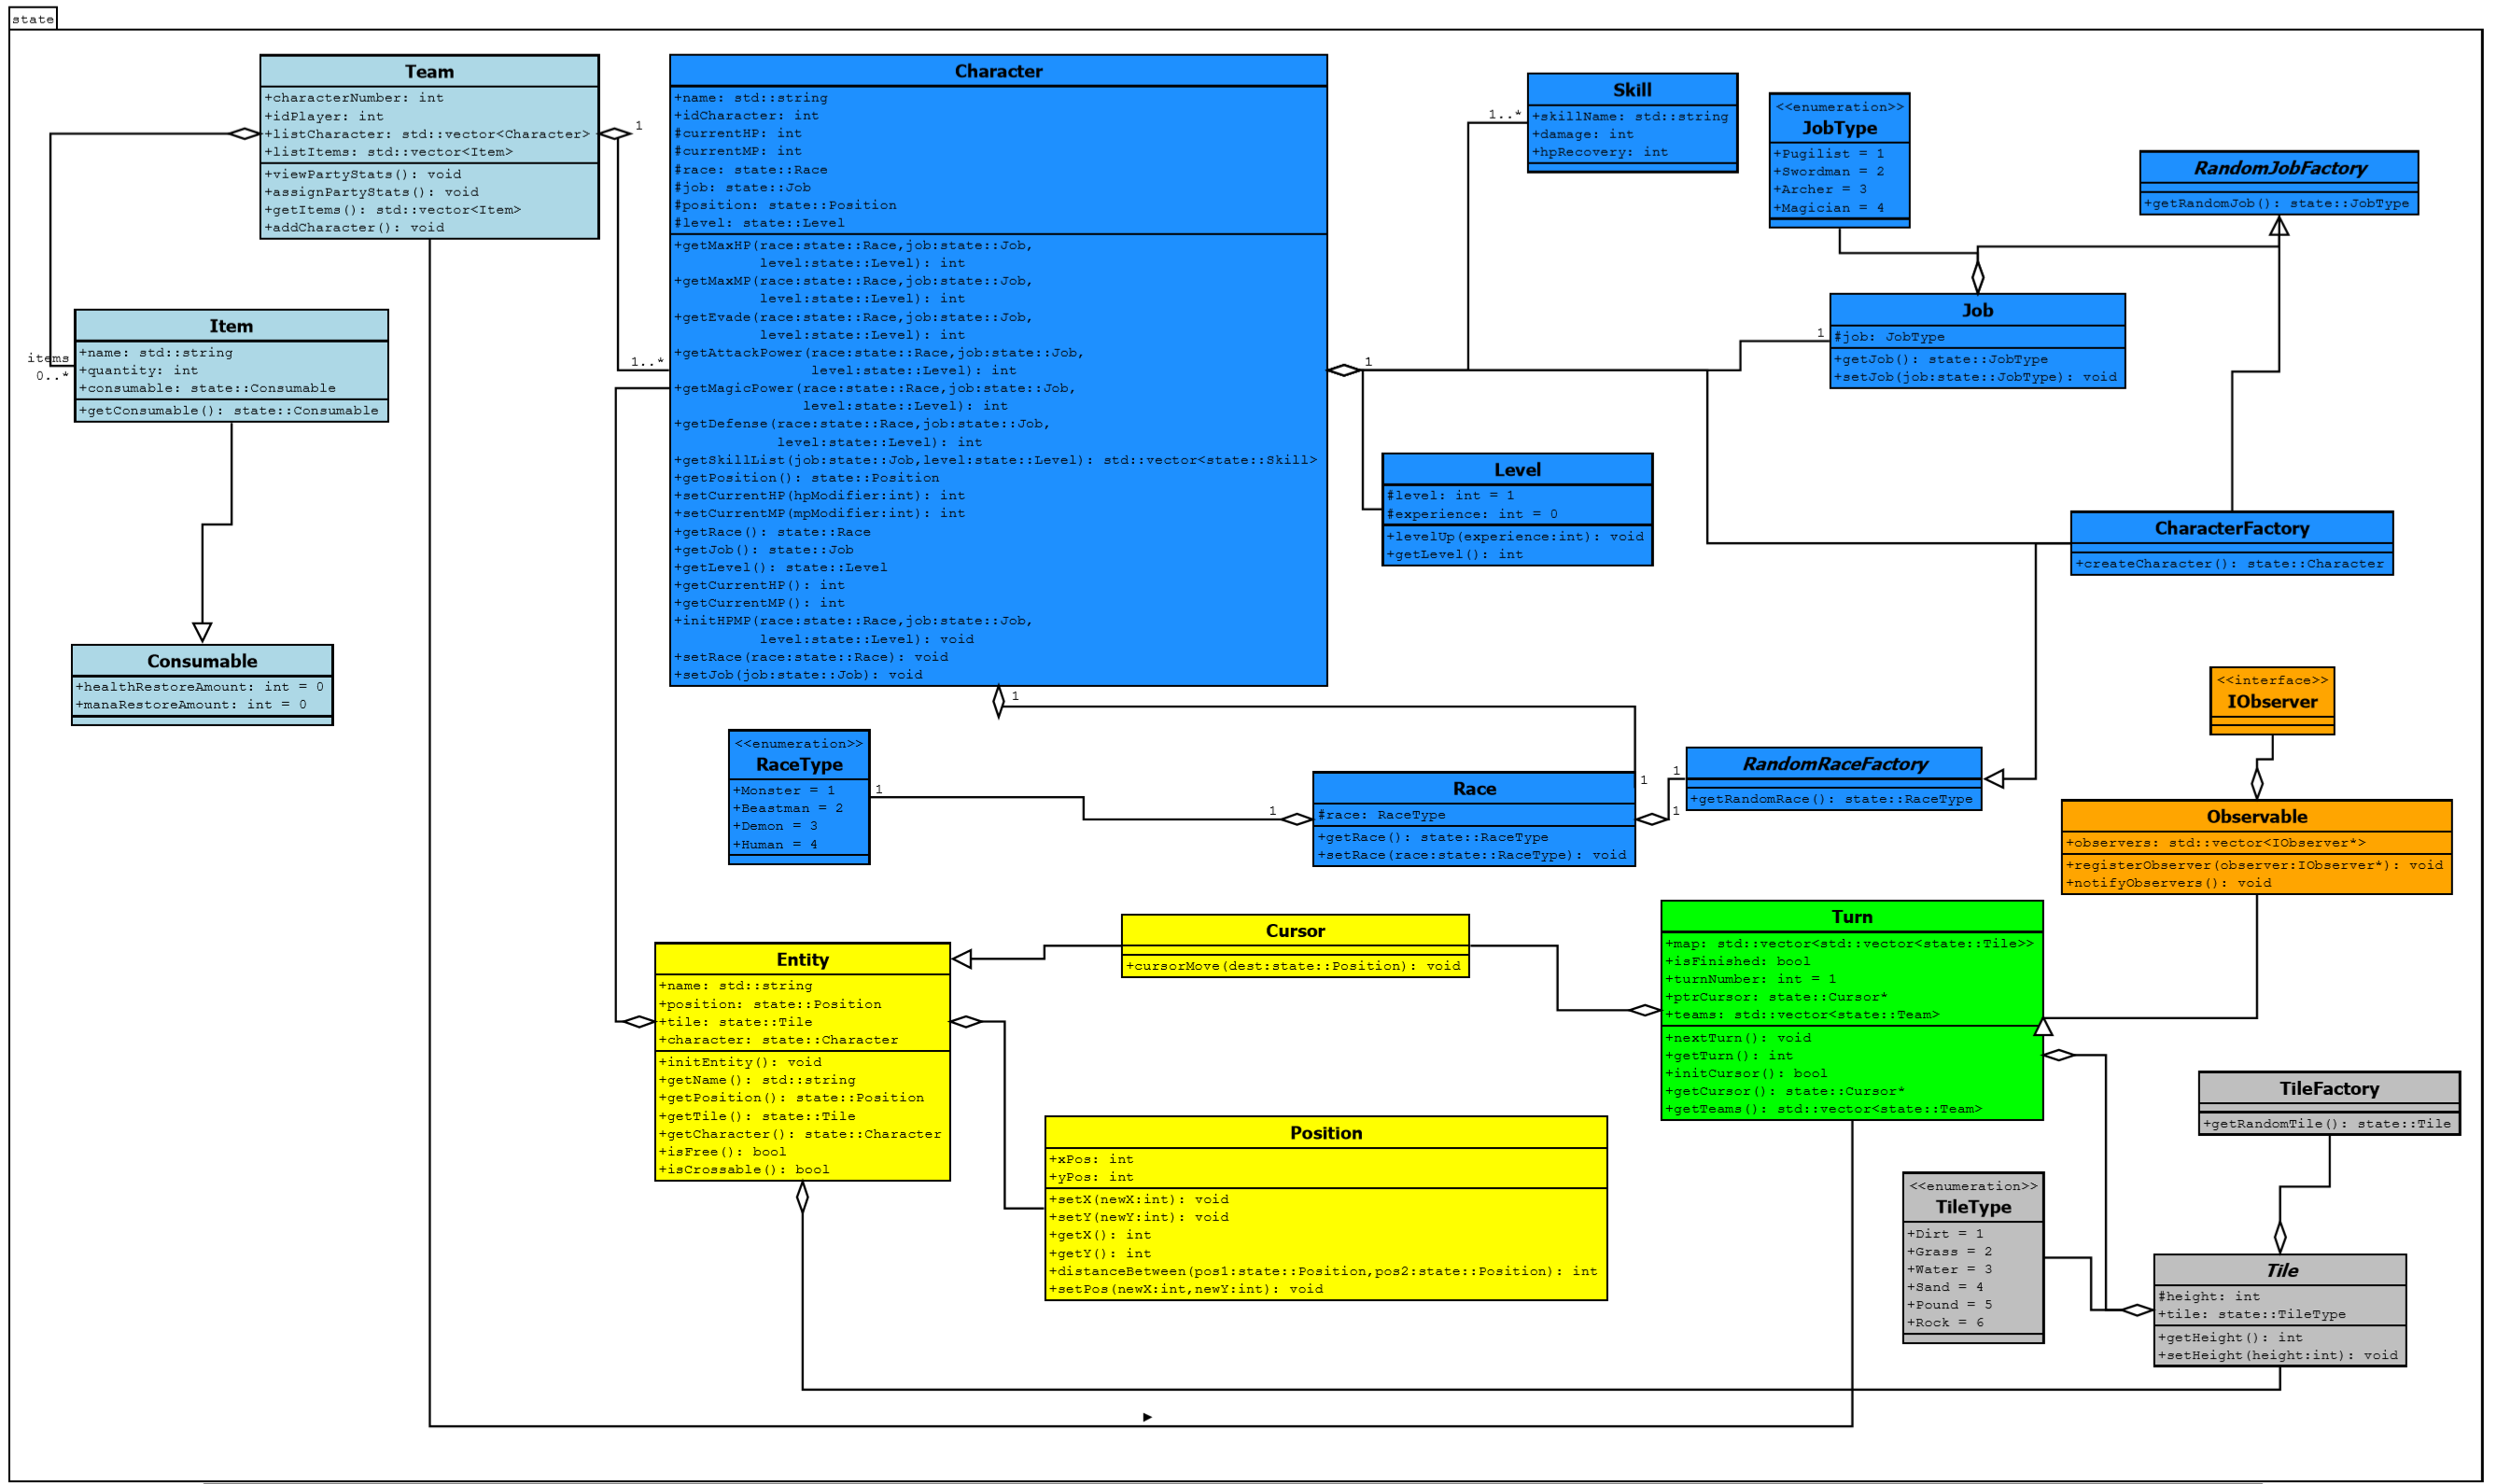
\includegraphics[width=\linewidth]{images/states.png}
\centering
\caption{Aperçu de state.dia}
\label{fig:img3}
\end{figure}
\newpage

\newpage

 \nocite{*}
%choix du style de la biblio
\bibliographystyle{plain}
%inclusion de la biblio
\bibliography{bibliographie}
%voir wiki pour plus d'information sur la syntaxe des entrées d'une bibliographie

\end{document}